    %------------------第二章---------------------------
    \newpage
	\section{超声波接近传感器原理与总体设计}
 \subsection{超声波接近传感器原理}

 
 \subsection{超声波接近传感器总体设计}
	在进行传感器各部分的设计之前,首先进行整体部分的设计,如图\ref{传感器整体设计}所示,可将传感器设计分为三个大部分:硬件设计、软件设计、实验设计。
\begin{figure}[ht]
	    \centering
	    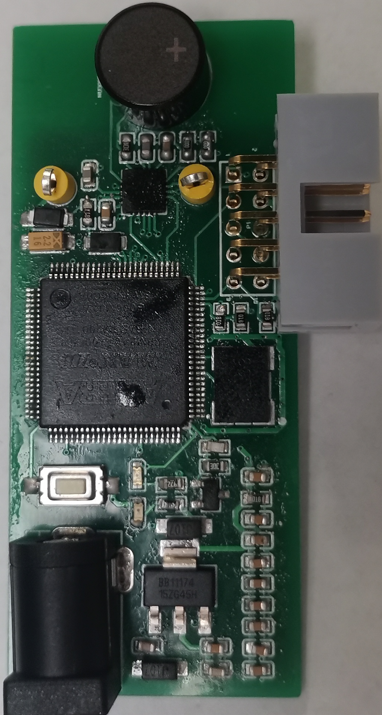
\includegraphics[width=8cm,angle=-90]{figure/physical map.png}
	    \caption{传感器整体设计}
	    \label{传感器整体设计}
\end{figure}

 \noindent
 \textbf{1、硬件设计}\par
硬件电路分为三部分来进行设计,分别为:CPLD芯片基本电路、TUSS4470芯片外围电路、检测计数电路。而CPLD芯片的电路又包括了电源电路、时钟电路、JTAG下载电路、复位电路。
其中设计难度最大的是TUSS4470芯片外围电路,需要通过查阅芯片手册来完成各个引脚的设计。\par
 \noindent
 \textbf{2、软件设计}\par
 传感器的软件设计根据功能分为了三个部分:SPI通信、脉冲产生、回波检测,其中SPI与脉冲发生部分需要根据芯片手册中的配置来进行程序算法设计。\par
 SPI通信选取的模式为CPOL=0、CPHA=1,采用全双工模式,程序通过使用线性序列机(linear sequential machine)来控制一个移位寄存器实现该逻辑。\par
 而脉冲产生则选择脉冲模式3,通过io1、io2两个引脚来配合控制产生脉冲。\par
 检测方面采用多次检测、判断次数的检测逻辑,以此来增加检测的稳定性。

 \noindent
 \textbf{3、实验设计}\par
 在完成实物的制作之后,需要设计实验来测试传感器的性能以及其检测逻辑的可行性。\par
 实验设计包括了设计实验测试传感器性能参数、设计实验测试其稳定性、设计实验测试不同材料的回波。
 
 